\documentclass[../main.tex]{subfiles}

\subsection{Rétegek}

\subsubsection{Perzisztencia réteg}

Legalsó réteg a perzisztencia, ahol a fájlok kezelése, mentése és betöltése történik.
Mivel a mentés osztályhierarchiába van szervezve, egy osztálynak elég megvalósítania a
\textit{QDataStreamSerializablen} interfészt ahhoz, hogy a perzisztencia osztály kezelni tudja.

\begin{center}
	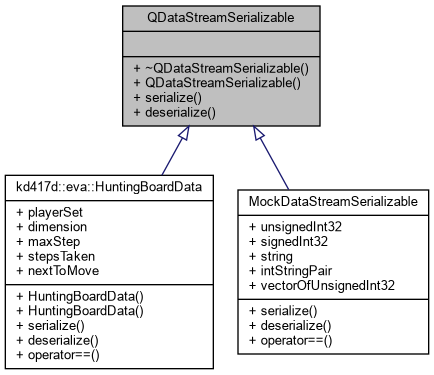
\includegraphics[width= 0.55\textwidth ]{structQDataStreamSerializable__inherit__graph.png}
\end{center}

A \textit{Serializer} osztálynak már csak a fájlkezelést kell végeznie, mivel a szerializációs
logikát egy osztály korábban megvalósította.

\begin{center}
	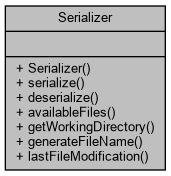
\includegraphics[width= 0.3\textwidth ]{classSerializer__coll__graph.png}
\end{center}

\subsubsection{Modell réteg}

A modell réteg egy metódusban elfedve kezeli a játék logikai részét.
Ehhez több "Utility" és egy főosztályba vannak szervezve a releváns metódusok.
A modell osztály logikai koordinátákkal dolgozik, melyeket 1-től indexelünk.
Minden adat, ami a modellben található, menthető egy adatosztályba, ami azután
szerializálható a perzisztencia rétegben.



\begin{multicols}{2}
	
\begin{center}
	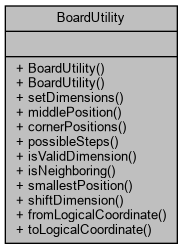
\includegraphics[width=0.25\textwidth]{images/classBoardUtility__coll__graph}
\end{center}

\begin{center}
	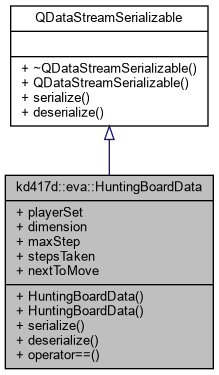
\includegraphics[width=0.3\textwidth]{structkd417d_1_1eva_1_1HuntingBoardData__coll__graph.png}
\end{center}

\columnbreak

	
\begin{center}
	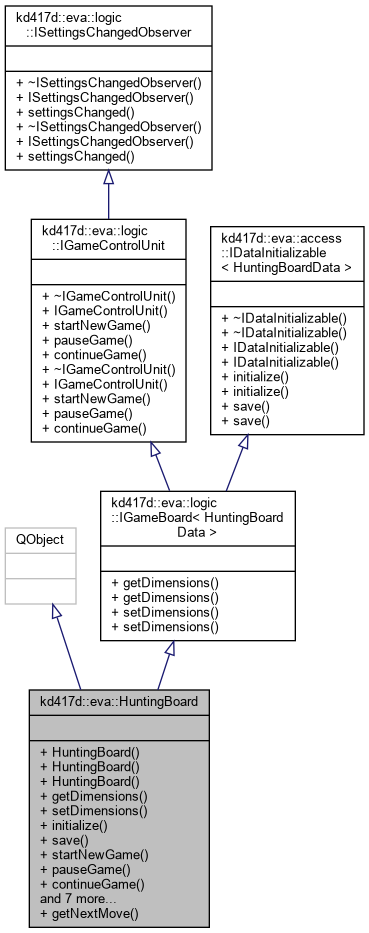
\includegraphics[width=0.4\textwidth]{classkd417d_1_1eva_1_1HuntingBoard__inherit__graph.png}
\end{center}

\end{multicols}{}

\textbf{Metódusok} \newline
A \textit{movePlayer} metódus segítségével kommunikál a nézet réteg a modell réteggel.
Ha egy játékos mozgatása sikeres, arról esemény ad tájékoztatást. \newline

\textbf{Adattagok} \newline
A \textit{mPlayerMap} adattagban vannak a játékosok, akik helyzete változhat, játékostípusuk
azonban soha. \newline 


\subsubsection{Nézet réteg}
A nézet réteg felelős a tábla eseményeinek megjelenítéséért. A tábla logikáját kirajzolva,
egy táblázatként jeleníti meg, ami minden lépésnél frissülés hatására újra kirajzolódik.
Ez a réteg felelős továbbá a felhasználó által mozgatni kívánt bábuk regisztrálásáért és továbbításáért
a modell réteg felé. Ezt az egér követésével valósítja meg.

\begin{center}
	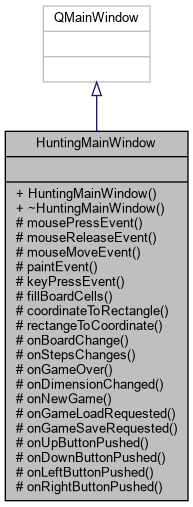
\includegraphics[width=0.25\textwidth]{classHuntingMainWindow__coll__graph.png}
\end{center}

\textbf{Adattagok} \newline
A \textit{} metódus segítségével kommunikál a nézet réteg a modell réteggel.
Ha egy játékos mozgatása sikeres, arról esemény ad tájékoztatást.

\subsubsection{Modell réteg teljes osztályhierarchiája}
\begin{center}
	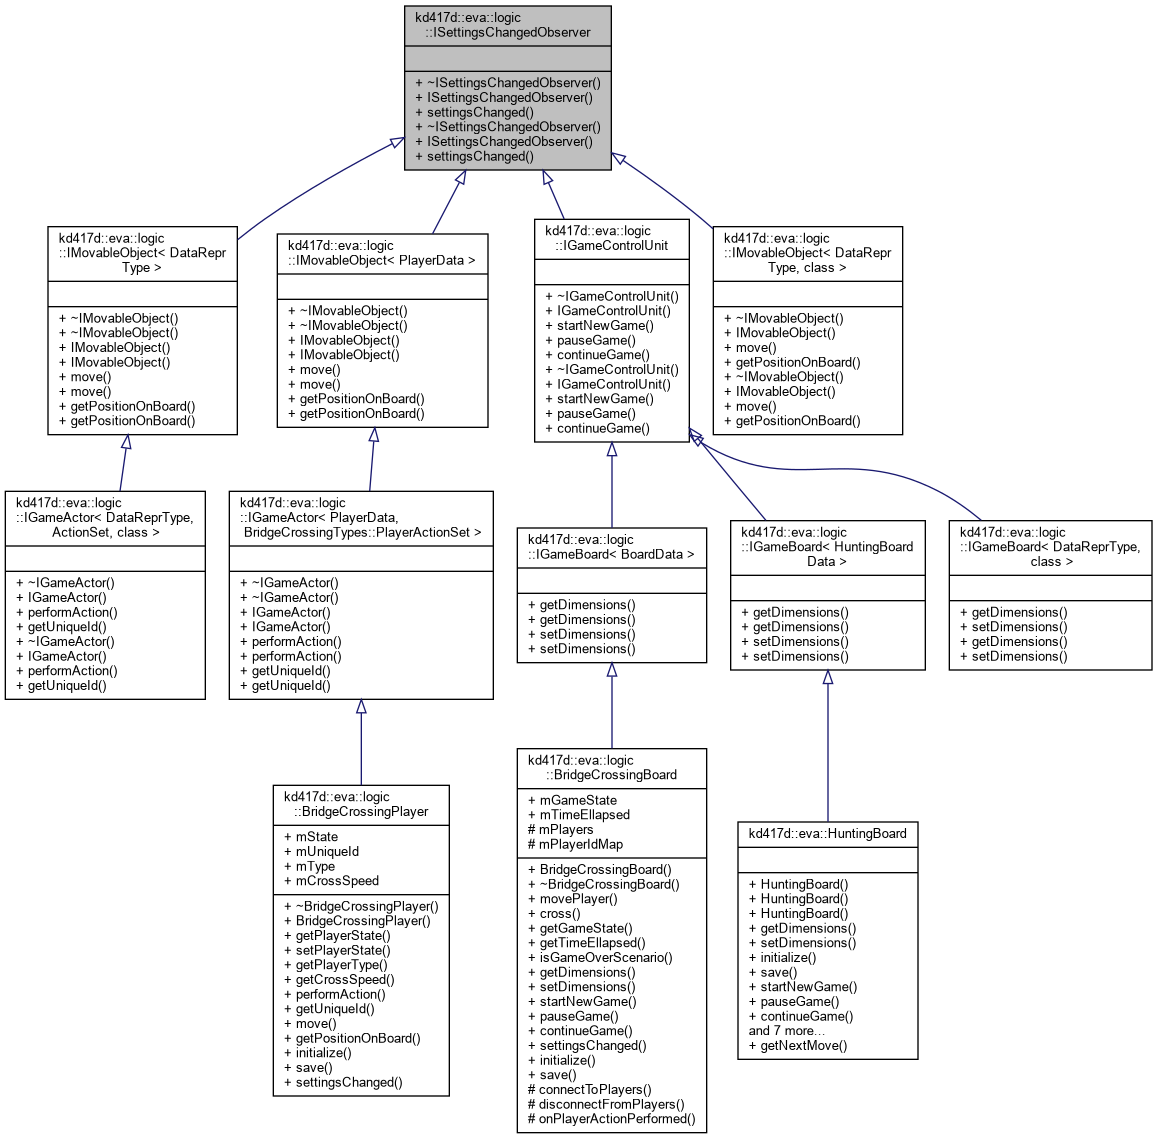
\includegraphics[width= 1\textwidth]{classkd417d_1_1eva_1_1logic_1_1ISettingsChangedObserver__inherit__graph.png}
\end{center} 	


\subsubsection{Eseménykezelés}

Eseménykezelés megvalósul a nézet-tábla között.
A nézet által kezelt nyomógombok a tábla bizonyos metódushívásait idézik elő.
Ezeket a hívásokat a tábla továbbítja a táblának, majd eseményben tájékoztatást
kap annak sikerességéről. Természetesen az is lehet, hogy a tábla által észlelt
lépés engedélyezett, de a jelenlegi játékállapot ezt nem teszi lehetővé (például az
adott pozíció már foglalt).

\begin{center}
\begin{tabular}{| c | c | c | c |}
    \hline
    \rowcolor{TableHeaderBlue}
    sender & signal & reciever & slot \\
    \hline
    HuntingBoard & newGameSignal & HuntingMainWindow & onNewGameStarted \\
    \hline
    HuntingBoard & boardChangedSignal & HuntingMainWindow & onBoardChanged \\
    \hline
    HuntingBoard & scoredPointChangedSignal & HuntingMainWindow & onScoredPointChanged \\
    \hline
    HuntingBoard & gameOverSignal & HuntingMainWindow & onGameOver \\
    \hline

\end{tabular}
\end{center}

